\documentclass[portuguese]{textolivre}

% metadata
\journalname{Texto Livre}
\thevolume{17}
%\thenumber{1} % old template
\theyear{2024}
\receiveddate{\DTMdisplaydate{2024}{2}{8}{-1}}
\accepteddate{\DTMdisplaydate{2024}{10}{22}{-1}}
\publisheddate{\DTMdisplaydate{2024}{11}{5}{-1}}
\corrauthor{Ana Paula Bernardo Mendonça}
\articledoi{10.1590/1983-3652.2024.51188}
%\articleid{NNNN} % if the article ID is not the last 5 numbers of its DOI, provide it using \articleid{} commmand 
% list of available sesscions in the journal: articles, dossier, reports, essays, reviews, interviews, editorial
\articlesessionname{articles}
\runningauthor{Mendonça e Alves}
%\editorname{Leonardo Araújo} % old template
\sectioneditorname{Daniervelin Pereira}
\layouteditorname{João Mesquita}

\title{Cursos Online Abertos e Massivos (MOOC) em contextos corporativos: uma revisão da literatura}
\othertitle{Massive Open Online Courses (MOOC) in corporate contexts: a literature review}

\author[1,2]{Ana Paula Bernardo Mendonça~\orcid{0000-0002-9873-3370}\thanks{Email: \href{mailto:anapaulabm@gmail.com}{anapaulabm@gmail.com}}}
\author[1]{Lynn Rosalina Gama Alves~\orcid{0000-0003-3688-3506}\thanks{Email: \href{mailto:lynnalves@gmail.com}{lynnalves@gmail.com}}}
\affil[1]{Programa de Gestão e Tecnologia Industrial no Senai/Cimatec, Salvador, Bahia, Brasil.}
\affil[2]{Fundação Oswaldo Cruz – Fiocruz, Rio de Janeiro, RJ, Brasil.}

\addbibresource{article.bib}

\usepackage{nameref}
\usepackage{array}

\begin{document}
\maketitle
\begin{polyabstract}
\begin{abstract}
Este estudo visa investigar como Cursos Online Abertos e Massivos (MOOC) vêm sendo adotados como espaços formativos em organizações, com enfoque em identificar as práticas e estratégias aplicadas para reduzir a evasão nesses cursos. Para atingir tal objetivo, foi realizada uma revisão sistematizada da literatura, consultando bases de dados como Web of Science, Scopus e SciELO, em busca de artigos relacionados ao tema publicados no período de 2018 a 2022. Após a aplicação dos critérios de inclusão e exclusão, apenas cinco artigos foram considerados relevantes, apontando a lacuna de pesquisas no campo. Os resultados destacam os MOOC como espaços formativos relevantes para qualificação e requalificação profissional em contextos corporativos. Identifica-se ainda sua contribuição para outras funções, incluindo gestão de carreira, recrutamento, retenção de talentos e marketing de produtos ou serviços.  Entretanto, um desafio significativo identificado é o de cultivar a motivação dos trabalhadores para conclusão dos cursos. Os resultados indicam a necessidade de promover o alinhamento entre as expectativas dos trabalhadores e metas organizacionais e de desenvolver estratégias que valorizem as necessidades individuais, a autonomia e o desempenho do aprendiz. Destacam-se estratégias como aprimorar a aprendizagem por meio de abordagens pedagógica adaptativa, assim com a promoção de incentivos monetários e não monetários para o reconhecimento pelo desempenho. O estudo identificou uma lacuna significativa na literatura: a ausência de estudos sobre os desafios da abordagem pedagógica autoinstrucional nos MOOC.

\keywords{MOOC \sep Educação Corporativa \sep Treinamento Profissional \sep Formação Profissional \sep Curso Virtual}
\end{abstract}

\begin{english}
\begin{abstract}
This study aims to investigate how Massive Open Online Courses (MOOC) have been adopted as formative spaces within organizations, with a focus on identifying the practices and strategies applied to reduce dropout rates in these courses. To achieve this goal, a systematic literature review was conducted, consulting databases such as Web of Science, Scopus, and SciELO, in search of articles related to the topic published between 2018 and 2022. After applying inclusion and exclusion criteria, only five articles were considered relevant, highlighting a research gap in the field. The results emphasize MOOCs as relevant formative spaces for professional qualification and requalification in corporate contexts. Their contribution to other functions, including career management, recruitment, talent retention, and the marketing of products or services, is also identified. However, a significant challenge identified is fostering workers' motivation to complete the courses. The results indicate the need to promote alignment between workers' expectations and organizational goals and to develop strategies that value individual needs, autonomy, and learner performance. Highlighted strategies include enhancing learning through adaptive pedagogical approaches, as well as the promotion of monetary and non-monetary incentives for performance recognition. The study identified a significant gap in literature: the absence of studies on the challenges of the self-instructional pedagogical approach in MOOC.

\keywords{MOOC \sep Corporate Education \sep Professional education \sep E-learning \sep Online Learning}
\end{abstract}
\end{english}
\end{polyabstract}

\section{Introdução}
Nas últimas duas décadas, observou-se um aumento expressivo na oferta de Cursos Online Abertos e Massivos (MOOC). Trata-se de um modelo de curso concebido para permitir o acesso a qualquer indivíduo interessado, independentemente de qualificações prévias, suportando milhares de participantes em uma única oferta \cite{yousef_reflections_2021}. 

Os MOOC incluem uma variedade de recursos educacionais, como vídeos, palestras, atividades de avaliação e fóruns de discussão que podem ser acessados a qualquer momento e em qualquer lugar, constituindo-se como uma opção conveniente e flexível para a qualificação ou requalificação profissional \cite{goglio_contribution_2021}. 

A ascensão dos MOOC foi marcada pela capacidade de suportar um exponencial número de participantes, desde os primeiros cursos de Stanford, em 2011, que receberam 300 mil alunos. Esse modelo de curso ganhou popularidade mundial a partir de 2012 com a criação das plataformas provedoras globais de MOOC, como Coursera. EdX e Udacity, entre outras \cite{pappano_year_2012}. Desde então, essas plataformas têm oferecido tanto cursos de curta duração quanto programas de certificação nos mais variados temas, desenvolvidos por universidades, instituições de ensino superior ou em colaboração com organizações profissionais e empresas de tecnologia, atraindo alunos que desejam alcançar potenciais benefícios de carreira \cite{goglio_contribution_2021}.

Em 2020, impulsionada pela pandemia, a procura desses cursos nas plataformas aumentou significativamente, com um acréscimo de 60 milhões de inscritos no ano \cite{shah_by_2021}. Em 2021, destacou-se a procura desses cursos por empresas e governos, direcionando o público dos MOOC para o ambiente corporativo. No Coursera, por exemplo, os cursos para empresas e governos são o segmento que mais cresce, com 70\% ao ano, contra 29\% relacionados aos procurados pelo público em geral \cite{shah_by_2021}.

Dessa forma, os MOOC se consolidaram como uma alternativa de aprendizagem sob demanda, visando suprir lacunas de habilidades no cenário profissional contemporâneo, onde as tecnologias digitais estão transformando indústrias e serviços, encurtando os ciclos de \textit{feedback} e criando setores que resultam em novas ou na obsolescência de funções. Essa tendência educacional reflete a necessidade proeminente de formação contínua ao longo da vida \cite{farrow_mooc_2018}, em consonância com as demandas do mercado atual por formação contínua.

Nesse cenário, esse modelo de curso se apresenta como um espaço formativo relevante para setores em que a escassez de habilidades são desafios significativos, particularmente em indústria de alta tecnologia, incluído serviços biomédicos, científicos, logística e tecnologia da informação \cite{rosendale_scaling_2021}.

No entanto, desde a sua criação, um desafio constante associado aos MOOC é a alta taxa de evasão nos cursos, em torno de 90\% \cite{bates_teaching_2019}.  A alta taxa de evasão pode ser atribuída a diversos fatores relatados por estudos como o de \textcite{tang_learning_2017,singh_analysis_2018,yousef_reflections_2021,gil-quintana_citizenship_2020}, tais como a conexão lenta de Internet,  níveis de letramento digital abaixo do esperado, a alta carga de atividades, o nível de complexidade dos conteúdos em relação aos diferentes públicos alcançados, a necessidade de auto-organização dos participantes, o sentimento de distância entre professor e aluno e a ausência ou atraso de \textit{feedback}.

Apesar da crescente adoção dos MOOC nos ambientes corporativos, sua exploração para fins de aprendizagem corporativa não tem sido amplamente pesquisada. Notadamente, existe uma escassez de estudos e evidências empíricas sobre as implicações dos MOOC sob uma perspectiva corporativa, contrastando com o elevado número de pesquisas sobre o impacto e eficácia dos MOOC no ensino superior e na educação de adultos em geral \cite{zur_transforming_2021,yan_construction_2022,park_moocs_2021}. Algumas das razões significativas incluem a novidade do fenômeno e sua recente tendência de adoção em ambientes corporativos. A adoção inicial desses cursos foi realizada por instituições de ensino como universidades, que naturalmente estimularam mais pesquisas nesse contexto. Outra questão pode estar relacionada a dificuldade de acesso a dados.  Empresas privadas podem ser relutantes em compartilhar dados sobre o uso de MOOC para treinamento interno devido a preocupações com privacidade, segurança de dados ou vantagem competitiva. Isso limita o acesso dos pesquisadores a informações detalhadas necessárias para estudar o impacto dos MOOC no contexto corporativo.

Por conseguinte, esta pesquisa visa investigar como os MOOC vêm sendo adotados como espaços formativos em organizações, identificando as práticas e estratégias aplicadas para reduzir a taxa de evasão nos cursos. Dessa forma, buscamos responder as seguintes questões: Como as empresas vêm tratando e discutindo a adoção dos MOOC como espaços formativos de seus trabalhadores? Quais práticas são adotadas para reduzir a taxa de evasão nos MOOC?

Este artigo está estruturado em quatro seções: além desta introdução, a seção \ref{sec-normas} descreve o desenho metodológico da pesquisa; a seção \ref{sec-formato} apresenta os resultados e a discussão dos estudos; e a seção \ref{sec-modelo} aborda as considerações finais com base na revisão da literatura realizada.

\section{Desenho metodológico}\label{sec-normas}
Nesta investigação, de abordagem qualitativa, realizamos uma revisão sistematizada da literatura. Diferente da revisão de literatura tradicional, que permite maior flexibilidade na elaboração e adaptação das diretrizes, a revisão sistematizada é caracterizada por um processo metodológico mais rígido e pré-definido.  Sobretudo, a presente revisão da literatura buscou fornecer uma visão abrangente do conhecimento existente sobre o fenômeno dos MOOC no contexto corporativo. Segundo \textcite{galvao_principais_2015}, uma revisão sistemática da literatura consiste em um processo rigoroso de pesquisar, selecionar, avaliar, sintetizar e relatar evidências a partir de uma pergunta bem estruturada. 

Dado ao tema emergente e ao objetivo da investigação, optamos por adotar o método de revisão sistematizada da literatura, considerado o mais adequado para resumir e sintetizar evidências sobre a eficácia e os efeitos de uma determinada intervenção \cite{sampaio_estudos_2007}.

Para tanto, o estudo foi dividido em duas fases, que apresentamos nas subseções a seguir: \Cref{sec-conduta} \nameref{sec-conduta} e \Cref{sec-fmt-manuscrito} \nameref{sec-fmt-manuscrito}. Os resultados e a discussão serão apresentados na \Cref{sec-formato} \nameref{sec-formato}.  


\subsection{Definição do tema e das questões da pesquisa}\label{sec-conduta}
A pesquisa concentra-se no tema dos MOOC aplicados em contextos corporativos. O objetivo dessa pesquisa é investigar como esse modelo de curso vem sendo adotado como espaços formativos em organizações, com enfoque em identificar as práticas e estratégias aplicadas para reduzir a taxa de evasão nesses cursos. 

É importante destacar que esses espaços formativos diferem dos processos educacionais formais promovidos pelas universidades. Para o contexto desta pesquisa, essas formações se referem ao processo de desenvolvimento de competências e habilidades que visam alcançar um determinado objetivo relacionado ao trabalho ou à carreira e se diferem dos processos educacionais que vão além da instrumentalização. Sobretudo, consideramos que um não exclui a importância do outro, mas se complementam para alcançar objetivos organizacionais e profissionais no contexto de trabalho ou de carreira.

Dessa forma, esse estudo busca responder as seguintes questões: Como as empresas vêm tratando e discutindo a adoção dos MOOC como espaços formativos de seus trabalhadores? Quais práticas são adotadas para reduzir a taxa de evasão nos MOOC?


\subsection{Pesquisas nas bases de dados científicas e análise dos estudos}\label{sec-fmt-manuscrito}
Após definir o tema e as questões de pesquisa, passamos à segunda fase, onde selecionamos as bases de dados científicas, as palavras-chave para a busca e os critérios de inclusão e exclusão. Nessa fase, elegemos as bases de dados Web of Science, Scopus, Scientific Electronic Library Online (SciELO) e ERIC. A escolha dessas bases de dados foi pautada pelo reconhecimento em termos de confiabilidade e pela amplitude de periódicos e publicações disponíveis. Especificamente, a base ERIC foi escolhida por seu foco em produções na área de educação.

Em seguida, definimos as palavras-chave “aprendizagem corporativa” e “MOOC”. Com as palavras-chave definidas, realizamos testes de buscas no Google Acadêmico aplicando as palavras-chave para identificar as variações dos termos e compor a \textit{string} de busca indicada a seguir: 

(corporat* OR organi* OR “corporate university” OR  "corporate education"  OR  "corporate Learning" OR “workplace learning” OR “professional learning”)  AND  (mooc  OR “massive course” "massive open online course")

Os asteriscos (*) após "corporat" e "organi" funcionam como curingas, significando que qualquer extensão dessas raízes de palavras será aceitável (por exemplo, "corporate", "corporation", "organizational", “organization” etc.). As frases entre aspas são tratadas como expressões exatas, então o motor de busca procurará por essas frases exatas no texto.

Como critérios de inclusão definimos: publicações de 2018 a 2022, revisados por pares nos idiomas português, inglês e espanhol, com acesso ao texto completo disponível pelo Portal de Periódicos Capes, incluindo artigos teóricos e empíricos. Para os critérios de exclusão, consideramos as publicações fora do escopo dos MOOC fora do contexto corporativo e àqueles que não se enquadraram nos critérios de inclusão como bibliografias, teses, dissertações, livros, capítulo de livros, editoriais, relatórios, resenhas, publicações com acesso fechado, texto escrito em idioma diferente dos citados, além das publicações duplicadas.  

A partir da \textit{string} e os critérios de inclusão e exclusão definidos, realizamos a busca manual nas bases de dados aplicando os filtros baseados nos critérios definidos. O processo de pesquisa nas bases de dados científicas e análise dos estudos foi realizado durante o mês de junho de 2022, consistindo em quatro etapas: identificação, triagem, elegibilidade e inclusão dos estudos na análise.   Os resultados dessas etapas e a discussão dos estudos analisados serão apresentados na próxima seção \ref{sec-formato}.


\section{Resultados e discussão}\label{sec-formato}
Na primeira etapa, identificamos 232 registros que foram importados para o software Zotero, onde excluímos 5 registros duplicados.  Na segunda etapa de triagem, os 227 registros restantes foram exportados do Zotero para a planilha do Excel. Após a exportação, procedemos a leitura dos títulos dos trabalhos, aplicando os critérios de inclusão e exclusão, resultando na exclusão de 198 estudos que estavam fora do escopo. Na terceira e última etapa, realizamos a leitura dos resumos e das palavras-chave dos 29 artigos restantes, para confirmar se atendiam ao critério de elegibilidade MOOC em contextos corporativos. Dessa forma, excluímos 24 estudos que não atenderam a esse critério. Ao final, cinco estudos foram considerados relevantes para leitura completa e todos foram incluídos na análise. Esta decisão está alinhada com o objetivo de cobrir as perspectivas existentes, apesar dos potenciais limitações metodológicas. Entendemos que os estudos ofereceram um panorama do estado atual do conhecimento e lacunas existentes na literatura sobre a aplicação de MOOC em contextos corporativos. A figura a seguir (\Cref{fig1}) mostra o fluxo das etapas realizadas:

\begin{figure}[h]
\centering
\begin{minipage}{0.75\linewidth}
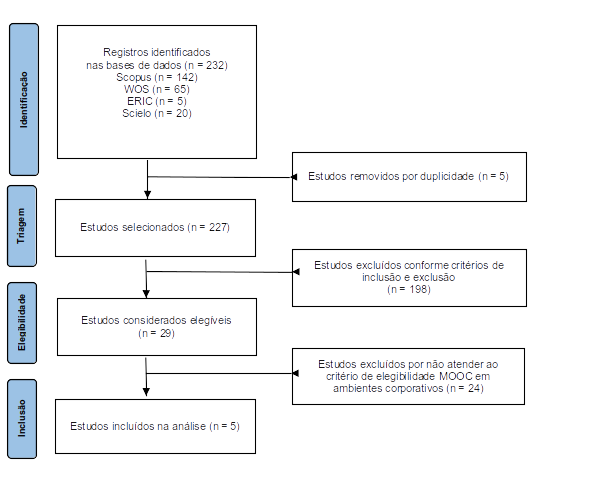
\includegraphics[width=\linewidth]{Fig1.png}
\caption{Fluxo das etapas das pesquisas nas bases de dados científicas e análise dos dados.}
\label{fig1}
\source{Elaborado pelas autoras.}
\end{minipage}
\end{figure}

Os estudos descritos na \Cref{tbl1} foram analisados criticamente no sentido de investigar como os MOOC vêm sendo adotados como espaços formativos em organizações, a fim de identificar as práticas e estratégias aplicadas para reduzir a evasão nesses cursos. Dessa forma, buscamos responder as seguintes questões: Como as empresas vêm tratando e discutindo a adoção dos MOOC como espaços formativos de seus trabalhadores? Quais práticas são adotadas para reduzir a taxa de evasão dos MOOC?

\begin{table}[h]
\centering
\begin{threeparttable}
\caption{Trabalhos incluídos na revisão da literatura..}
\label{tbl1}
\begin{tabular}{>{\raggedright\arraybackslash}p{3cm} >{\raggedright\arraybackslash}p{5cm} >{\raggedright\arraybackslash}p{3cm}}
\toprule
Autores & Título & Periódico \\ 
\midrule
\textcite{park_moocs_2021} & MOOC in the workplace: an intervention for strategic human resource development & Human Resource Development International \\ 
\textcite{becerra_diseno_2020} & Diseño pedagógico adaptativo para el desarrollo de MOOC: uma estrategia para el desarrollo de competencias en contextos corporativos & Revista Electronica de Investigacion Educativa \\
\textcite{sureephong_effect_2020} & The effect of non-monetary rewards on employee performance in massive open online courses & International Journal of Emerging Technologies in Learning \\
\textcite{zur_transforming_2021} & Transforming workplace learning: A qualitative inquiry into adopting massive open online courses into corporate learning and development & Education Sciences \\
\textcite{yan_construction_2022} & Construction and Application of Vocational Training Platform for Enterprise Employees & Mobile Information Systems \\
\bottomrule
\end{tabular}
\source{Elaboração própria.}
\end{threeparttable}
\end{table}

Particularmente, a adoção dos MOOC é notada em corporações globais, com exemplos de empresas de diferentes setores da indústria \cite{park_moocs_2021} e em países com setores industriais robustos, como a China \cite{yan_construction_2022} e Tailândia \cite{sureephong_effect_2020}. Além disso, um dos estudos relatou a experiência de formações oferecidas pelo governo em larga escala para servidores públicos \cite{becerra_diseno_2020}.

Empresas como Adidas, McAfee, Deutsche Telekom, Google e L'Oréal foram mencionadas como exemplos de organizações que adotaram amplamente o modelo de MOOC, com destaque para a SAP. A SAP, uma empresa líder no setor de tecnologia da informação, é reconhecida como pioneira na adoção deste modelo de curso como estratégia de aprendizagem digital. Desde 2013, a empresa mantém uma plataforma corporativa de MOOC, oferecendo mais de 280 cursos em uma variedade de tópicos específicos e gerais. Essa plataforma já registrou mais de 700.000 inscrições de alunos \cite{zur_transforming_2021}. 

Nesse cenário, os MOOC são empregados em uma variedade de propósitos além do treinamento, incluindo gestão de talentos, recrutamento, marketing para fortalecimento de marca e fomento da colaboração entre diferentes setores e indústrias.  No entanto, em consonância com as constatações de autores como \textcite{zur_transforming_2021,yan_construction_2022,park_moocs_2021}, existe uma escassez de pesquisas sobre os MOOC aplicados em contextos corporativos, como se revelou na prospecção realizada na presente pesquisa. Adicionalmente destacamos a ausência de estudos brasileiros nesse contexto. 

Embora a pesquisa sobre MOOC ainda esteja em uma fase exploratória, os resultados apontam que sua adoção vem refletindo a necessidade de formação contínua diante do aumento da complexidade das atividades organizacionais, especialmente no contexto das atuais mudanças tecnológicas e econômicas \cite{zur_transforming_2021}.

Existe um consenso entre os pesquisadores analisados de que os MOOC constituem uma estratégia relevante para empresas interessadas em expandir as opções e o alcance de treinamentos. Esses cursos podem preencher lacunas de competências e habilidades da força de trabalho, contribuindo assim para o alcance dos objetivos organizacionais \cite{becerra_diseno_2020,zur_transforming_2021,yan_construction_2022,park_moocs_2021}. 

De acordo com \textcite{yan_construction_2022}, as empresas estão integrando MOOC aos programas de treinamento presenciais para criar uma abordagem híbrida - \textit{online-to-offline} (O2O). A abordagem O2O combina a conveniência da aprendizagem assíncrona dos MOOC com a flexibilidade de outras atividades educacionais, que podem ser realizadas tanto de forma síncrona online quanto presencialmente. As atividades síncronas podem incluir \textit{workshops}, sessões práticas ou treinamentos em grupo. O objetivo é promover uma imersão que aplique os conhecimentos adquiridos online, maximizando assim o impacto dos MOOC \cite{yan_construction_2022}.

O autor argumenta que os MOOCs têm o potencial de diminuir os custos relacionados a treinamentos presenciais, uma vez que eliminam despesas com deslocamento e hospedagem. Além disso, esses cursos online permitem a realização de treinamentos em larga escala e de forma simultânea, possibilitando a participação de trabalhadores independentemente de onde estejam localizados. Isso amplia significativamente o alcance das iniciativas de desenvolvimento pessoal nas organizações \cite{yan_construction_2022}.

O primeiro aspecto relacionado a adoção de MOOC e uma prática a ser considerada para reduzir a evasão relaciona-se ao alinhamento estratégico dos MOOC aos objetivos gerais da organização. Nesse sentido, \textcite{park_moocs_2021} argumentam que os MOOC alinhados estrategicamente com os objetivos do departamento de recursos humanos, podem ir além dos treinamentos, expandindo-se para outras áreas do desenvolvimento de recursos humanos, como a retenção de talentos, o desenvolvimento organizacional e de carreira. Neste estudo, os autores analisaram três casos de organizações que alinharam o uso de MOOC às suas estratégias organizacionais como a Microsoft, Tenaris e o banco indiano Axis Bank que merecem destaque:
 
A Microsoft empregou MOOC para implementar mudanças organizacionais e treinar sua equipe de vendas, apoiando a inovação em seus modelos de negócios, alcançando taxas de conclusão de 85\%, com avaliação de 95\% no grau de satisfação entre os trabalhadores. 

O Axis Bank, enfrentando alta rotatividade e buscando reter talentos, reformulou seu sistema de gestão de desempenho para enfatizar a aprendizagem e o desenvolvimento como estratégia central. O banco adotou a plataforma Coursera para oferecer aos funcionários cursos em uma variedade de tópicos, incluindo liderança, análise de dados e conhecimentos bancários. Os cursos foram personalizados para atender às necessidades específicas da empresa, permitindo que os funcionários os escolhessem com base em suas necessidades individuais.

A Tenaris, reconhecendo que programas pontuais de formação eram insuficientes, redefiniu seu modelo de formação. Através de sua Universidade Corporativa, alinhou os cursos às metas de desempenho da empresa, alcançando uma taxa de conclusão de 90\% \cite{park_moocs_2021}.

\textcite{park_moocs_2021} também notaram que algumas empresas ao disponibilizar seus cursos publicamente, os utilizam como estratégia de marketing e recrutamento para atrair uma ampla gama de participantes, incluindo usuários, clientes e parceiros. Dessa forma, utilizam os MOOC tanto para promover seus produtos quanto para identificar talentos para recrutamento. Um exemplo notável é o da Google, que adotou o modelo MOOC para programas de certificação global. Estes programas visam capacitar usuários, identificar potenciais talentos, bem como capacitar os membros da equipe de suporte para os produtos da Google Cloud Platform. 

\textcite{park_moocs_2021} concluíram que a adoção dos MOOC deve estar vinculada aos objetivos estratégicos das organizações para melhorar a performance dos resultados e, ao mesmo tempo, diminuir a taxa de evasão dos cursos. Contudo, é importante notar que a pesquisa tem suas limitações, incluindo a ausência de entrevistas com trabalhadores ou outras partes interessadas nas organizações estudadas, o que poderia fornecer insights adicionais sobre a implementação e o impacto dos MOOC

\textcite{zur_transforming_2021} conduziram 36 entrevistas com gestores corporativos, responsáveis pelas práticas de aprendizagem e desenvolvimento em organizações de diferentes setores da indústria.  Os entrevistados reconheceram que os MOOC podem promover a autonomia do aprendiz, manter as habilidades e o conhecimento profissional dos funcionários atualizados e ampliar o acesso a novos conhecimentos. A maioria dos entrevistados compreende os MOOC uma modalidade de aprendizagem complementar a modalidade presencial. Os gerentes também acreditam que os cursos apresentam vantagens em relação a outros modelos de treinamento devido a economia de custos e a possibilidade de realizar a jornada de aprendizagem de forma flexível e mais conveniente para o participante.

Embora essas expectativas sejam positivas, os autores ressaltam que a implementação de MOOC envolve várias dimensões que inclui a seleção de uma plataforma segura de dados, a definição de métricas para monitoramento das iniciativas e o acompanhamento do desempenho e da aprendizagem. Também é fundamental definir metas e expectativas claras sobre a adoção de MOOC e os resultados esperados. Além disso, as organizações devem considerar os custos associados ao acesso e uso das plataformas, bem como a necessidade de serviços intermediários para ajudar os gestores a desenvolverem cursos adequados para seus funcionários. Isso pode ser realizado por meio de funcionários com experiência em MOOC ou por consultorias externas, exigindo dos gestores proficiência na gestão desses processos \cite{zur_transforming_2021}.

\textcite{zur_transforming_2021} também enfatizam a importância de escolher plataformas que garantam a segurança e a confidencialidade dos dados da empresa e dos funcionários. Avaliar os resultados de cursos realizados em plataformas externas apresenta desafios adicionais, destacando a necessidade de uma análise cuidadosa da infraestrutura tecnológica e das implicações de segurança, privacidade, confidencialidade e confiabilidade. 

Segundo \textcite{dijck_data_2017}, as plataformas de MOOC, através do processo de datificação, geram e armazenam uma vasta quantidade de dados, possibilitando o uso de Inteligência Artificial, como análise preditiva e aprendizagem para compreender e otimizar a experiência educacional. No entanto, conforme Alves (2022), os sistemas de governança interna das plataformas, que incluem termos de uso e algoritmos, não são neutros e podem influenciar os resultados. Os algoritmos, muitas vezes operando como 'caixas pretas', podem levar a resultados seletivos e manipulados \cite{knox_beyond_2018}. Portanto, a resistência das empresas em adotar MOOC pode estar principalmente relacionada à preocupação com a segurança dos dados. 

Embora vantagens sejam percebidas, os MOOC frequentemente enfrentam altas taxas de desistência, o que pode ser um desafio para as organizações que desejam garantir a participação dos funcionários em tais cursos \textcite{sureephong_effect_2020,becerra_diseno_2020,yan_construction_2022}. 

\textcite{yan_construction_2022}, assim como \textcite{sureephong_effect_2020} sustentam que, no ambiente corporativo, a participação voluntária dos colaboradores em treinamentos não é suficiente para alcançar os objetivos das empresas. Para esses autores, é essencial, além do alinhamento estratégico, levar em conta um segundo aspecto: a motivação dos trabalhadores para concluir os cursos, que pode ser significativamente aumentada através de incentivos. Estes incentivos podem variar, sendo tanto de natureza monetária quanto não monetária.

\textcite{yan_construction_2022} recomenda que as empresas encontrem um equilíbrio entre os objetivos divergentes e conflitos de interesse entre as três partes envolvidas (empresas, departamentos de treinamento e colaboradores) ao implementar plataformas de formação profissional. Além disso, é recomendável que as empresas construam um mecanismo de incentivo razoável para o treinamento e desenvolvimento dos colaboradores. 

Nesse sentido, \textcite{yan_construction_2022} propõe a criação de um mecanismo de incentivo que aloca um valor de pagamento por desempenho para os trabalhadores que participam do treinamento MOOC e geram resultados. Isso pode significar oferecer oportunidades de progresso na carreira, bônus ou aumentos salariais para aqueles que completam com sucesso os cursos ou alcançam metas de desempenho. No entanto, \textcite{yan_construction_2022} ressalta a importância de proporcionar condições para que o trabalhador possa equilibrar o tempo dedicado ao treinamento e trabalho sugerindo estratégias como horários de trabalho flexíveis e suporte durante o treinamento. 

\textcite{sureephong_effect_2020}, por outro lado, investigaram o impacto de diferentes tipos de recompensas não monetárias na motivação e no desempenho dos funcionários em MOOC. O estudo foi realizado com 90 funcionários voluntários de uma empresa de fabricação de alimentos na Tailândia (Chiang Mai). Os pesquisadores empregaram a teoria de Instrumentalidade e Expectativa de Valência (VIE) para avaliar a motivação em três grupos de recompensas: Recompensas Não Monetárias Tangíveis, Recompensas Não Monetárias Sociais e Recompensas Não Monetárias Relacionadas ao Trabalho. Os resultados indicaram que as recompensas não monetárias tangíveis foram mais eficazes para aumentar a motivação dos funcionários e as taxas de conclusão do curso em MOOCs.

No primeiro experimento, com a utilização de questionário, foram avaliados os três tipos de recompensas não monetárias. As recompensas tangíveis incluem premiações com produtos, serviços ou viagens de férias; as recompensas sociais estão relacionadas ao relacionamento das pessoas dentro da organização, como reconhecimento público, entre outros; e, por último, as recompensas relacionadas ao trabalho, incluem oportunidades de em programas de treinamento, viagens de trabalho internacionais, horários de trabalho flexíveis e dias de folga.  

O segundo experimento visou descobrir qual tipo de recompensa não monetária é mais adequado para motivar os funcionários a participarem e concluir o curso. Os resultados mostraram que o grupo de recompensas não monetárias tangíveis atingiu a pontuação mais alta.  Cerca de 60\% dos participantes expostos a esse tipo de recompensa completaram os cursos \cite{sureephong_effect_2020}.   

O estudo de \textcite{sureephong_effect_2020} apresenta limitações significativas. Realizado com uma amostra específica e limitada de funcionários de uma empresa de alimentos na Tailândia, os resultados podem não ser generalizáveis para outros contextos. Além disso, o foco exclusivo em recompensas não monetárias, sem considerar recompensas monetárias ou a interação entre ambas, pode limitar a compreensão do espectro completo de motivações dos funcionários. A pesquisa também não aborda as variações individuais na percepção dessas recompensas e não explora a sustentabilidade de seus efeitos a longo prazo, além de depender da precisão das medidas de desempenho dos participantes. 

Da mesma maneira, o estudo de \textcite{yan_construction_2022} considerou somente as recompensas monetárias, carecendo, portanto, de uma análise comparativa entre esses tipos de incentivo.  Além disso, outras variáveis que podem afetar a motivação e o desempenho dos participantes nos cursos, como a cultura organizacional, o clima de trabalho, liderança, precisam ser observadas. Em última análise, considerações éticas e de equidade são fundamentais para evitar disparidades, garantindo que tais sistemas beneficiem todos os trabalhadores de maneira equânime.

Um terceiro aspecto citado como desafiador em termos motivacionais em ambientes de aprendizagem online massivos é a natureza assíncrona dos MOOC.  De acordo \textcite{park_moocs_2021}, pode haver atrasos no \textit{feedback}, o que pode afetar a eficácia do aprendizado e o envolvimento dos participantes, provocando o abandono nos cursos. 

Por outro lado, \textcite{becerra_diseno_2020} consideram que o problema da elevada taxa de evasão dos MOOC está a dificuldade de um curso massivo atender às demandas específicas dos trabalhadores. Para esses autores, o conteúdo padronizado desses cursos nem sempre está adequado ao público de destino. Desta forma, perceberam a necessidade de avançar para modelo de MOOC com desenho pedagógico adaptativo.  

A conceituação de adaptação para o estudo de \textcite{becerra_diseno_2020} está relacionada ao fato de que a aprendizagem, para ser bem-sucedida, deve oferecer diferentes alternativas de abordagens de um tema, de organização de conteúdo, explicações, representações e exemplos, além de materiais variados considerando o nível de formação, a diversidade cultural e a necessidade de adaptação dos conteúdos para garantir a inclusão máxima dos participantes.

Nesse sentido, \textcite{becerra_diseno_2020} estabeleceram um modelo pedagógico para MOOC que enfoca o desenvolvimento de competências aplicadas ao contexto de trabalho. Neste estudo, os cursos de formação tecnológica foram destinados a 1300 funcionários públicos de entidades estatais colombianas. O modelo incluiu a metodologia de Aprendizagem Baseada em Problemas (ABP), experiências de aprendizagem por meio de laboratórios práticos, recursos de gamificação para verificar o avanço dos participantes no curso e mecanismos para interação, como fóruns de discussão. 

O modelo pedagógico se concentrou em estratégias didáticas baseadas em situações reais, como estudos de caso, para promover o desenvolvimento de competências tecnológicas e de gestão institucional. A intenção do modelo foi enfatizar o aprendizado situado a partir de experiências de aprendizagem significativas e aplicáveis ao contexto real dos participantes \cite{becerra_diseno_2020}.

A proposta foi considerada bem-sucedida devido à taxa de abandono inferior a 60\%. Os autores defendem a importância de coletar \textit{feedback} dos participantes e da capacidade de adaptar as práticas de acordo com a necessidade dos funcionários, assim como fornece recursos adequados às realidades dos participantes.  O desenvolvimento do modelo envolveu a participação de diversos profissionais, como especialistas no tema, designers pedagógicos, designers gráficos, programadores e gestor de projetos \cite{becerra_diseno_2020}.

No entanto, implementar esse modelo em grandes grupos pode ser um desafio, por isso é importante que os professores desenvolvam habilidades digitais para usar efetivamente os recursos em suas práticas de ensino. Mediar as atividades propostas requer competências digitais dos professores e o desenvolvimento desses cursos envolve uma equipe especialista multidisciplinar \cite{becerra_diseno_2020}.

Contudo, a evolução de tecnologias como a Inteligência Artificial (IA), especialmente as versões generativas, tem contribuído para o surgimento de novas possibilidades de adaptação de conteúdos às necessidades dos participantes. Essas possibilidades são fortalecidas pelas práticas de \textit{Learning Analytics} (Análise da Aprendizagem, em português), que já vinham sendo utilizadas, marcando assim o início de um novo campo de estudo. 

A LA possibilita o monitoramento de diversas ações dos indivíduos em um curso (cliques em \textit{links}, tempo de interações, níveis de envolvimento, entre outras) e análise de seus contextos. Dessa forma, é possível, por meio da LA, identificar padrões de comportamento, alertar os alunos e professores sobre possíveis desistências, medir e subsidiar novas práticas para otimização da aprendizagem e dos ambientes em que ela ocorre, além de responder a uma infinidade de perguntas sobre como os indivíduos aprendem e interagem \cite{siemens_learning_2013}.

O uso de tecnologias emergentes como IA oferece diversas vantagens como a aprendizagem adaptativa, em tempo real, por meio de algoritmo de aprendizado por reforço e técnicas de análise de dados (LA). Monitorar o progresso dos alunos e ajustar automaticamente o ritmo e o conteúdo de acordo com as características individuais e dificuldades dos alunos \cite{altaleb_enhancing_2023}. Realizar a análise de comportamento e prevenção de abandono, promovendo intervenções específicas de incentivo. Prover sistemas de apoio a tutoria por meio de algoritmos de aprendizado de máquina que analisam o desempenho e as interações dos alunos, oferecendo \textit{feedback} em tempo real. Oferecer sugestões de materiais de estudo \cite{becerra_diseno_2020}. Recomendar pares para otimizar a formação dos grupos mais adequados para resultar em uma colaboração efetiva \cite{ma_effects_2023}.

Em contraponto, os cursistas estão sob total vigilância dos seus traços deixados no ambiente de aprendizagem. Estudos sugerem a importância da transparência e da explicação das decisões de IA para garantir a confiança dos usuários \cite{swamy_trusting_2023}. Para pequenas empresas, a implementação dessas tecnologias está restrita às limitações de recursos e infraestrutura \cite{bhatt_artificial_2023}. Portanto, a implementação de IA e LA envolve questões complexas, que vão desde desafios de infraestrutura, técnicos e éticos até questões práticas de adaptação ao contexto organizacional.

Embora essas tecnologias tenha avançado, a motivação para participação ainda é uma questão central dos MOOC apontada pela literatura. No entanto, pesquisadores como \cite{knox_beyond_2018} criticam considerar motivado somente os concluintes do curso, pois esse indicador rejeita as diferenças e considera os alunos que participam pouco como "anormais" e "desmotivados", rotulando-os negativamente. De acordo com o autor, essa abordagem é uma forma de regulação do externo e desconhecido, que não leva em consideração as diferenças e contextos dos alunos.  Nesse sentido, considerar as taxas de conclusão como um indicador de sucesso pode ser um equívoco, já que os participantes que concluem os curso podem não representar a maioria.

De fato, em sua maioria, as tecnologias de IA e LA para a aprendizagem, está reduzida a questões ao fator de desempenho e métodos de aprimorar a transmissão de conteúdo. Pouco se sabe acerca de estratégias didático-pedagógicas e tecnologias eficazes para estimular a interação entre os participantes em práticas colaborativas e ajudar o professor na tarefa de \textit{feedback} para alunos em curso massivos. 

Mediante a rápida evolução da IA, as pesquisas nesses tópicos sob a perspectiva organizacional são incipientes, carecendo de estudos.  Nesse sentido, nenhum estudo analisado considerou as implicações de fenômenos relacionados a vigilância proporcionada pela LA e o processo da datificação das plataformas. Portanto, mais estudos sobre o uso dessas tecnologias, privacidade e segurança de dados em plataformas MOOC são esperados.

Certamente os MOOC são importantes e possuem vantagens, contudo, as possíveis consequências negativas mediante sua adoção precisam ser criticamente avaliadas.  Nesse contexto, é importante considerar que as empresas possuem realidades diferentes e podem encontrar desafios como a falta de recursos financeiros ou tecnológicos para implementar uma plataforma própria devido aos custos associados a manutenção de infraestrutura ou contratação de serviços das plataformas MOOC ou intermediários.

Autores como \textcite{adam_digital_2019}, tem levantado a questão de países do Sul Global não participarem da produção de MOOC em grandes plataformas, afirmando que as limitações são estruturais. As Plataformas, como a EdX, por exemplo, exigem taxas de parceria exorbitantes, enquanto o Future Learn aceita apenas as 200 melhores universidades (a maioria ocidentais), com poucas exceções. Além disso, os custos de produção da criação de um MOOC significam que universidades menos ricas não podem participar. Em alguns casos, são feitas parcerias com universidades do Norte Global, o que pode levar a relações de poder desiguais.

\textcite{adam_digital_2019} ressalta o potencial dano causado pelas Plataformas de MOOC na perpetuação de epistemologias centradas no Ocidente e na marginalização de sistemas de conhecimento locais e indígenas, destacando que apesar de se apresentarem como uma forma de ampliar o acesso ao conhecimento global, esses cursos podem perpetuar relações desiguais. Portanto, é necessário encontrar um equilíbrio entre as oportunidades oferecidas pelos MOOC e os danos que eles podem causar negligenciando as realidades distintas dos trabalhadores e que precisam ser consideradas.

Para as organizações com menos recursos, os gestores podem adotar MOOC por meio de curadoria, selecionando cursos gratuitos disponíveis na Internet para recomendar aos funcionários. No entanto, a curadoria enfrenta o desafio para encontrar cursos que se alinhem perfeitamente com os valores, a cultura e os objetivos organizacionais \cite{zur_transforming_2021,yan_construction_2022}. 

Outro fator impeditivo para a implementação dos MOOC por curadoria nos países em desenvolvimento, como o Brasil e os países da África, é a barreira do idioma. Deve-se notar que muitas plataformas MOOC conhecidas foram desenvolvidas em inglês, o que é um desafio para muitos países em que a maioria da população não domina o idioma \cite{adam_digital_2019}. Ao contrário do que se prometia, as plataformas provedoras de MOOC podem contribuir ainda mais para a exclusão social, um problema que os criadores dos MOOC pretendiam superar \cite{goglio_contribution_2021}.

Pequenas e médias organizações enfrentam uma série de desafios na implementação de MOOC, principalmente devido às limitações financeiras, infraestruturais e de expertise técnica. Essas dificuldades indicam a necessidade de alternativas de baixo custo e de maior apoio estrutural e apoio governamental para que essas organizações possam se beneficiar das plataformas de MOOC. 

Por fim, consideramos que enquadrar tecnologias como disruptivas ou salvadoras, como destacado \textcite{knox_beyond_2018}, significa restringir-se à visão do "solucionismo tecnológico" é abandonar completamente o objetivo de uma transformação equitativa e qualitativa na educação.

\section{Considerações finais}\label{sec-modelo}
A revisão da literatura conduzida neste estudo ofereceu uma visão abrangente sobre a adoção de Cursos Online Abertos e Massivos (MOOC) em organizações, focando nas práticas e estratégias para mitigar a evasão. Os resultados evidenciam os MOOC como estratégias educacionais valiosas, adotadas por organizações para diversificar opções de treinamento e preencher lacunas de competências.

Essa adoção é particularmente notável em corporações globais, abrangendo não apenas o treinamento, mas também a gestão de talentos e o fortalecimento da marca. O sucesso dessas iniciativas depende de um planejamento cuidadoso e de investimentos em serviços especializados.

Embora os MOOC se mostrem promissores devido a flexibilidade, o maior desafio para as empresas é motivar os trabalhadores a concluírem os cursos. Nesse sentido, os resultados indicam a necessidade de promover o alinhamento entre as expectativas dos trabalhadores e metas organizacionais, desenvolver mecanismos de incentivo que recompense ao desempenho dos trabalhadores e aprimorar a aprendizagem por meio de modelo de curso que se adaptem as necessidades e diferentes realidades dos participantes. 

Os MOOC representam uma área fértil para investigações futuras sobre a sua sustentabilidade a longo prazo e o impacto real no desempenho dos trabalhadores e das organizações. Nesse sentido, recomendamos pesquisas sobre a aplicação de análises de dados e avaliação do desempenho dos participantes, bem como a influência de diferentes tipos de incentivos na motivação dos funcionários.

Identificamos uma lacuna significativa na literatura: a ausência de estudos acerca de estratégias didático-pedagógicas e tecnologias eficazes para estimular a interação entre os participantes em práticas colaborativas e ajudar o professor na tarefa de \textit{feedback} para alunos em curso massivos. Assim, abrimos caminho para um campo robusto de futuras investigações que podem enriquecer a compreensão e eficácia dos MOOC no contexto corporativo.

O estudo possui limitações devido a análise foi circunscrita a um corpus limitado de artigos, uma consequência direta da natureza emergente do tema investigado. Esta emergência, por sua vez, restringiu a disponibilidade de publicações extensivas na área, resultando em uma seleção de artigos predominantemente em inglês, com uma notável ausência de estudos em português. Tal limitação linguística pode ter implicado na exclusão de perspectivas que poderiam enriquecer o entendimento do fenômeno estudado. Ademais, a concentração em artigos acadêmicos, embora metodologicamente justificável, pode ter restringido o espectro de análise, excluindo potencialmente outras formas de publicações científicas, como livros e capítulos de livros, que poderiam oferecer \textit{insights} adicionais. Esta escolha metodológica, necessária para delimitar o escopo do estudo, deve ser considerada ao interpretar as conclusões alcançadas.



\printbibliography\label{sec-bib}
%conceptualization,datacuration,formalanalysis,funding,investigation,methodology,projadm,resources,software,supervision,validation,visualization,writing,review
\begin{contributors}[sec-contributors]
\authorcontribution{Ana Paula Bernardo Mendonça}[conceptualization,writing]
\authorcontribution{Lynn Rosalina Gama Alves}[conceptualization,review]
\end{contributors}
\end{document}
